\documentclass[a4paper,x11names]{article}
% Here there is a bug that using \usepackage[x11names]{xcolor} would cause "Package xcolor Error: Undefined color `tikz@color".
% According to https://tex.stackexchange.com/questions/124636/package-xcolor-error-undefined-colors-maroon-royal-blue-when-master-has-pdf,
% adding "x11names" option in documentclass instead could solve this issue.
\usepackage{amsmath,amssymb,geometry,graphicx,pgfplots,tikz,xcolor}
% \usepackage{algorithmic,amsthm,amsfonts,array,auto-pst-pdf,babel,biblatex,bm,booktabs,caption,cases,clrscode3e,color,csvsimple}
% \usepackage{dejavu,DejaVuSansMono,diagbox,enumerate,epstopdf,fancyhdr,float,hanging,hyperref,indentfirst}
% \usepackage{listings,makecell,makeidx,mips,multicol,multirow,natbib,parskip,rotating}
% \usepackage{setspace,siunitx,subfigure,tabularx,titlesec,tocbibind,ulem,url,vmargin}
% \usepackage[T1]{fontenc}
% \captionsetup[figure]{labelsep=period}
% \captionsetup[table]{labelsep=period}
\geometry{left=3.5cm,right=3.5cm,top=3.3cm,bottom=3.3cm}
\renewcommand\thesection{\arabic{section}}
% \setlength{\parindent}{2em}
% Preamble:
\pgfplotsset{compat=1.17}
\begin{document}
\begin{center}
\huge
\textbf{VE320\\Intro to Semiconductor Devices\\}
\Large
\vspace{30pt}
\uppercase{Homework 2}\\
\vspace{5pt}\today\\
\vspace{5pt}
Yihua Liu 518021910998
\vspace{5pt}
\rule[-10pt]{.97\linewidth}{0.05em}
\end{center}

1. The graph of $E_g$ versus T over the range $0\leq T\leq600K$ is shown in Figure 1.

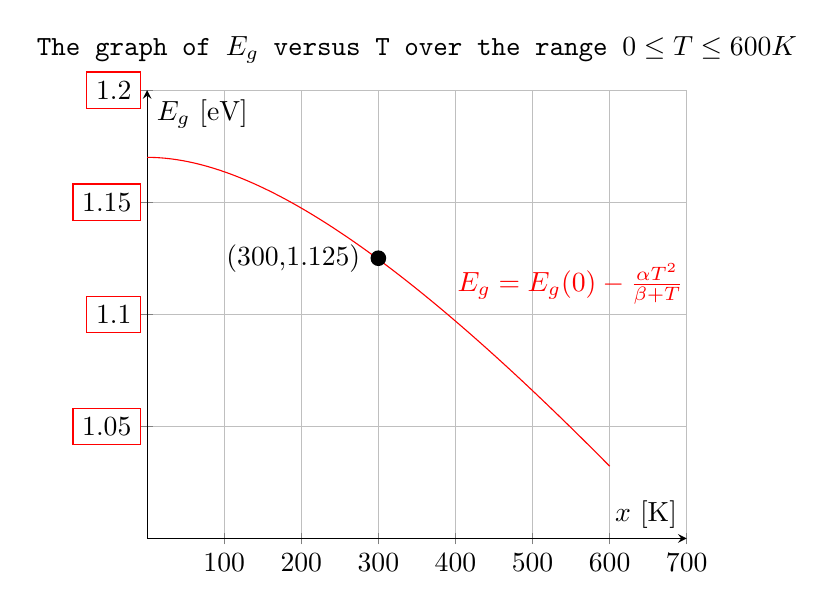
\begin{tikzpicture}
    \begin{axis}[
        title=\texttt{The graph of $E_g$ versus T over the range $0\leq T\leq600K$},
        ylabel={$E_g$ [eV]},
        every axis y label/.style={
            at={(ticklabel cs:0.5)},rotate=90,anchor=center,
        },
        % clip=false,     % to display the \path below
        ylabel style={draw=red},
        yticklabel style={draw=red},
        axis lines=center,
        xmax=700,
        ymin=1.0,
        ymax=1.2,
        xlabel={$x$ [K]},
        % use units,
        % x unit=K,
        % y unit=eV,
        % grmin=0:700 1:1.2,
        grid=major,
    ]
        \addplot[domain=0:600,samples=1000,red]
            {1.170-4.73*10^(-4)*x^2/(636+x)}
            % node [pos=1] (endofplotsquare) {};
            node [pos=0.65,above right] {$E_g=E_g(0)-\frac{\alpha T^2}{\beta+T}$};
        % \node [above,color=Firebrick2] at (endofplotsquare) {$E_g=E_g(0)-\frac{\alpha T^2}{\beta+T}$};
        \node[label={180:{(300,1.125)}},circle,fill,inner sep=2pt] at (axis cs:300,1.125) {};
        % \addplot[mark=*] coordinates {(300,0)} node[pin=150:{$(300,1.125)$}] {};
    \end{axis}
    % \draw[very thin,color=gray] (-0.1,-1.1) grid (3.9,3.9);
    % \draw[->] (-0.2,0) -- (4.2,0) node[right] {$x$};
    % \draw[->] (0,-1.2) -- (0,4.2) node[above] {$f(x)$};
    % \draw[color=red]    plot (\x,{1.170\times1.602176565\times10^{-19}+\x})        node[right] {$f(x) = }
\end{tikzpicture}

The value at $T$ = 300 K is
$$E_g=1.170-\frac{4.73\times10^{-4}T^2}{636+T}=1.170-\frac{4.73\times10^{-4}\times(300)^2}{636+300}=1.125\ \text{eV}.$$

2. (a) Using
$$\frac{1}{\hbar^2}\frac{\mathrm{d}^2E}{\mathrm{d}k^2}=\frac{2C_1}{\hbar^2}=\frac{1}{m^*},$$
at position A and D,
$$\frac{\mathrm{d}^2E}{\mathrm{d}k^2}<0,$$
the sign of the effective mass is negative;

at position B and C,
$$\frac{\mathrm{d}^2E}{\mathrm{d}k^2}>0,$$
the sign of the effective mass is positive.

(b) Using
$$\frac{1}{\hbar^2}\frac{\mathrm{d}E}{\mathrm{d}k}=\frac{p}{m}=v,$$
at position A and B,
$$\frac{\mathrm{d}E}{\mathrm{d}k}<0,$$
the direction of velocity for a particle is -$x$;

at position C and D,
$$\frac{\mathrm{d}E}{\mathrm{d}k}>0,$$
the direction of velocity for a particle is +$x$.

3. Using
$$\frac{1}{\hbar^2}\frac{\mathrm{d}^2E}{\mathrm{d}k^2}=\frac{2C_1}{\hbar^2}=\frac{1}{m^*},$$
we have
$$C_1=\frac{E}{k^2}.$$
Thus,
$$
\begin{aligned}
    C_1&=\frac{0.05\ \text{eV}}{(0.08\times10^{10}\ \text{m}^{-1})^2}\\
    &=1.252\times10^{-38}\ \text{kg}\cdot\text{m}^4\cdot\text{s}^{-2}.
\end{aligned}
$$
The effective mass of the electron in material A is
$$m^*=\frac{\hbar^2}{2C_1}=\frac{\hbar^2k^2}{2E}=4.442\times10^{-31}\ \text{kg}.$$
Denote the free electron mass as $m_e$. The effective mass in units of the free electron mass of the electron in material A is
$$m^*=\frac{m^*m_e}{m_e}=\frac{\hbar^2k^2m_f}{2Em_e}=0.488m_e.$$
Similarly, the effective mass of the electron in material B is
$$m^*=\frac{\hbar^2}{2C_2}=\frac{\hbar^2k^2}{2E}=4.442\times10^{-32}\ \text{kg}.$$
The effective mass in units of the free electron mass of the electron in material B is
$$m^*=\frac{m^*m_e}{m_e}=\frac{\hbar^2k^2m_f}{2Em_e}=0.0488m_e.$$

4. (a) (i) The frequency
$$\nu=\frac{E}{h}=\frac{1.42\times e}{h}=3.434\times10^{14}\ \text{Hz}.$$
Thus, the minimum frequency of an incident photon that can interact with a valence electron and elevate the electron to the conduction band is $3.434\times10^{14}$ Hz.

(ii) The wavelength
$$\lambda=\frac{c}{\nu}=\frac{hc}{E}=\frac{hc}{1.42\times e}=8.731\times10^{-7}\ \text{m}.$$
Thus, the corresponding wavelength is $8.731\times10^{-7}$ m.

(b) (i) The frequency
$$\nu=\frac{E}{h}=\frac{1.12\times e}{h}=2.708\times10^{14}\ \text{Hz}.$$
Thus, the minimum frequency of an incident photon that can interact with a valence electron and elevate the electron to the conduction band is $2.708\times10^{14}$ Hz.

(ii) The wavelength
$$\lambda=\frac{c}{\nu}=\frac{hc}{E}=\frac{hc}{1.42\times e}=1.107\times10^{-6}\ \text{m}.$$
Thus, the corresponding wavelength is $1.107\times10^{-6}$ m.

5. The effective mass at $k=k_0$ can be calculated by
\begin{equation}
    \frac{1}{\hbar^2}\frac{\mathrm{d}^2E}{\mathrm{d}k^2}\bigg|_{k=k_0}=\frac{1}{m^*}.
\end{equation}
Given $E=E_0-E_1\cos{\alpha(k-k_0)}$, the first derivative of the energy is
$$\frac{\mathrm{d}E}{\mathrm{d}k}=\alpha E_1\sin{\alpha(k-k_0)}.$$
The second derivative of the energy is
$$\frac{\mathrm{d}^2E}{\mathrm{d}k^2}=\alpha^2E_1\cos{\alpha(k-k_0)}.$$
At $k=k_0$,
$$\frac{\mathrm{d}^2E}{\mathrm{d}k^2}=\alpha^2E_1.$$
Substituting $\frac{\mathrm{d}^2E}{\mathrm{d}k^2}$ in Eq. (1),
$$m^*=\frac{\hbar^2}{\alpha^2E_1}.$$
Therefore, the effective mass of the particle at $k=k_0$ in terms of the equation parameters is $\frac{\hbar^2}{\alpha^2E_1}$.
\end{document}